\documentclass[aspectratio=169,11pt]{beamer}

% =========================================================
% FRC weekly group-meeting update
% Juan Pablo Solis Ruiz --- 22 September 2026
% =========================================================

% ---------- Theme ----------
\usetheme{Boadilla}
\usecolortheme{default}
\setbeamertemplate{navigation symbols}{}

% Show only the current slide number
\setbeamertemplate{footline}{%
  \leavevmode%
  \hbox{%
    \begin{beamercolorbox}[wd=.92\paperwidth,ht=2.4ex,dp=1.0ex,leftskip=.35cm]{author in head/foot}%
      \usebeamerfont{author in head/foot}\color{mygray}\scriptsize FRC Simulation Research --- Week 2 Update
    \end{beamercolorbox}%
    \begin{beamercolorbox}[wd=.08\paperwidth,ht=2.4ex,dp=1.0ex,center]{date in head/foot}%
      \usebeamerfont{date in head/foot}\color{mygray}\scriptsize\insertframenumber
    \end{beamercolorbox}%
  }%
}

% ---------- Packages ----------
\usepackage[utf8]{inputenc}
\usepackage[T1]{fontenc}
\usepackage{lmodern}
\usepackage{amsmath,amssymb}
\usepackage{graphicx}
\usepackage{xcolor}
\usepackage{booktabs}
\usepackage{array}
\usepackage{ragged2e}
\usepackage{hyperref}

% ---------- Figure paths ----------
\graphicspath{{img/audit/FRC_baseline_audit/}{img/audit/FRC_spatial_baseline/}}

% ---------- Colors ----------
\definecolor{myblue}{RGB}{20,45,90}
\definecolor{midblue}{RGB}{43,86,145}
\definecolor{lightblue}{RGB}{231,239,249}
\definecolor{lightgray}{RGB}{244,246,248}
\definecolor{mygray}{RGB}{75,75,75}
\definecolor{goodgreen}{RGB}{58,117,92}
\definecolor{softgreen}{RGB}{232,243,237}
\definecolor{accentgold}{RGB}{157,111,31}
\definecolor{softgold}{RGB}{249,243,229}

\hypersetup{
    colorlinks=true,
    urlcolor=myblue,
    linkcolor=myblue
}

\setbeamercolor{title}{fg=myblue}
\setbeamercolor{frametitle}{fg=white,bg=myblue}
\setbeamerfont{frametitle}{series=\bfseries,size=\large}
\setbeamercolor{structure}{fg=myblue}
\setbeamercolor{normal text}{fg=black,bg=white}
\setbeamercolor{author in head/foot}{fg=mygray,bg=white}
\setbeamercolor{date in head/foot}{fg=mygray,bg=white}
\setbeamercolor{block title}{fg=white,bg=midblue}
\setbeamercolor{block body}{fg=black,bg=lightblue}

\setbeamercolor{donebox}{fg=black,bg=softgreen}
\setbeamercolor{workbox}{fg=black,bg=lightblue}
\setbeamercolor{nextbox}{fg=black,bg=softgold}
\setbeamercolor{neutralbox}{fg=black,bg=lightgray}

\setbeamertemplate{frametitle}{%
  \nointerlineskip
  \begin{beamercolorbox}[wd=\paperwidth,ht=2.8ex,dp=1.2ex,leftskip=0.4cm]{frametitle}
    \usebeamerfont{frametitle}\insertframetitle
  \end{beamercolorbox}
}

% ---------- Convenience macros ----------
\newcommand{\smallcapslabel}[1]{%
    {\scriptsize\bfseries\color{myblue}\MakeUppercase{#1}}%
}

\newcommand{\statusbox}[3]{%
    \begin{beamercolorbox}[wd=\linewidth,rounded=true,sep=0.58em]{#1}
        {\scriptsize\bfseries #2}\par
        \vspace{0.04cm}
        {\scriptsize #3}
    \end{beamercolorbox}%
}

\newcommand{\source}[1]{%
    \vspace{0.04cm}\par{\raggedleft\tiny\color{mygray}#1\par}%
}

% ---------- Title Info ----------
\title{FRC Simulation Research}
\subtitle{Inherited Baseline Audit and Framework Direction}
\author{Juan Pablo Solís Ruiz}
\institute{University of Science and Technology of China (USTC)\\Supervisor: Prof. Ren Haijun}
\date{Group Meeting --- 22 September 2026}

\begin{document}

% =========================================================
\begin{frame}[plain]
    \vspace{0.70cm}
    {\color{myblue}\LARGE\bfseries FRC Simulation Research}\par
    \vspace{0.16cm}
    {\Large Inherited Baseline Audit and Framework Direction}\par
    \vspace{0.48cm}

    \begin{beamercolorbox}[wd=0.92\textwidth,rounded=true,sep=0.80em]{block body}
        \smallcapslabel{Current focus}\par
        \vspace{0.10cm}
        Characterize the inherited WarpX FRC baseline before building an independent, reproducible case-management workflow.
    \end{beamercolorbox}

    \vfill
    {\large\textbf{Juan Pablo Solís Ruiz}}\\[0.08cm]
    {\normalsize USTC --- Plasma / Fusion Research Group}\\[0.08cm]
    {\small Supervisor: Prof. Ren Haijun}\\[0.08cm]
    {\small 22 September 2026}
    \vspace{0.30cm}
\end{frame}

\setcounter{framenumber}{0}

% =========================================================
\begin{frame}
\frametitle{This Week: Practical Takeover of the Inherited Baseline}

\begin{columns}[T,totalwidth=\textwidth]
    \begin{column}{0.50\textwidth}
        \smallcapslabel{Main progress}
        \vspace{0.06cm}
        \begin{beamercolorbox}[wd=\linewidth,rounded=true,sep=0.55em]{donebox}
        \small
        \begin{itemize}\setlength\itemsep{0.12cm}
            \item Accessed the SCNet environment and identified the inherited FRC/WarpX working directories.
            \item Preserved the original directories as a read-only reference.
            \item Built a separate workspace: \texttt{FRC\_jpsr}.
            \item Set up a Python analysis environment and compiled \texttt{yt} locally to read WarpX/AMReX plotfiles.
        \end{itemize}
        \end{beamercolorbox}
    \end{column}

    \begin{column}{0.48\textwidth}
        \smallcapslabel{Baseline status}
        \vspace{0.06cm}
        \begin{beamercolorbox}[wd=\linewidth,rounded=true,sep=0.55em]{block body}
        \small
        \begin{itemize}\setlength\itemsep{0.12cm}
            \item Legacy executable: 3D WarpX, MPI + OpenMP, CPU backend.
            \item Two inherited reference runs: \texttt{i} and \texttt{j}.
            \item Both use the same physical input; differences are due to independent PIC realizations.
            \item Existing baseline duration: \(2~\mu\mathrm{s}\), shorter than the imposed \(4~\mu\mathrm{s}\) field-rise time.
        \end{itemize}
        \end{beamercolorbox}
    \end{column}
\end{columns}

\vspace{0.16cm}
\begin{beamercolorbox}[wd=\textwidth,rounded=true,sep=0.44em]{nextbox}
{\scriptsize\textbf{Goal:} turn the inherited case into a documented regression baseline before modifying or extending the workflow.}
\end{beamercolorbox}

\end{frame}

% =========================================================
\begin{frame}
\frametitle{Scalar Audit: Runs \texttt{i} and \texttt{j} Agree Macroscopically}

\begin{columns}[T,totalwidth=\textwidth]
    \begin{column}{0.58\textwidth}
        \begin{minipage}{0.49\linewidth}
            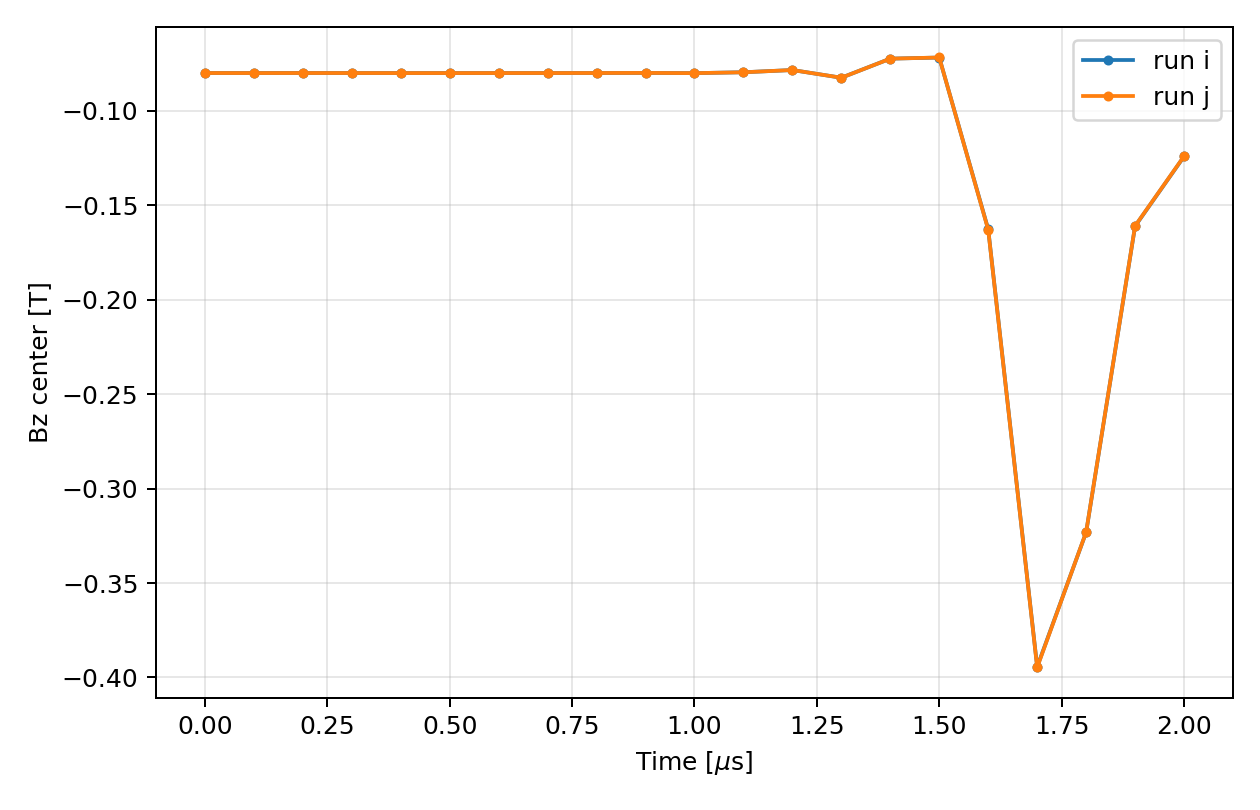
\includegraphics[width=\linewidth]{Bz_center_vs_time.png}
        \end{minipage}
        \hfill
        \begin{minipage}{0.49\linewidth}
            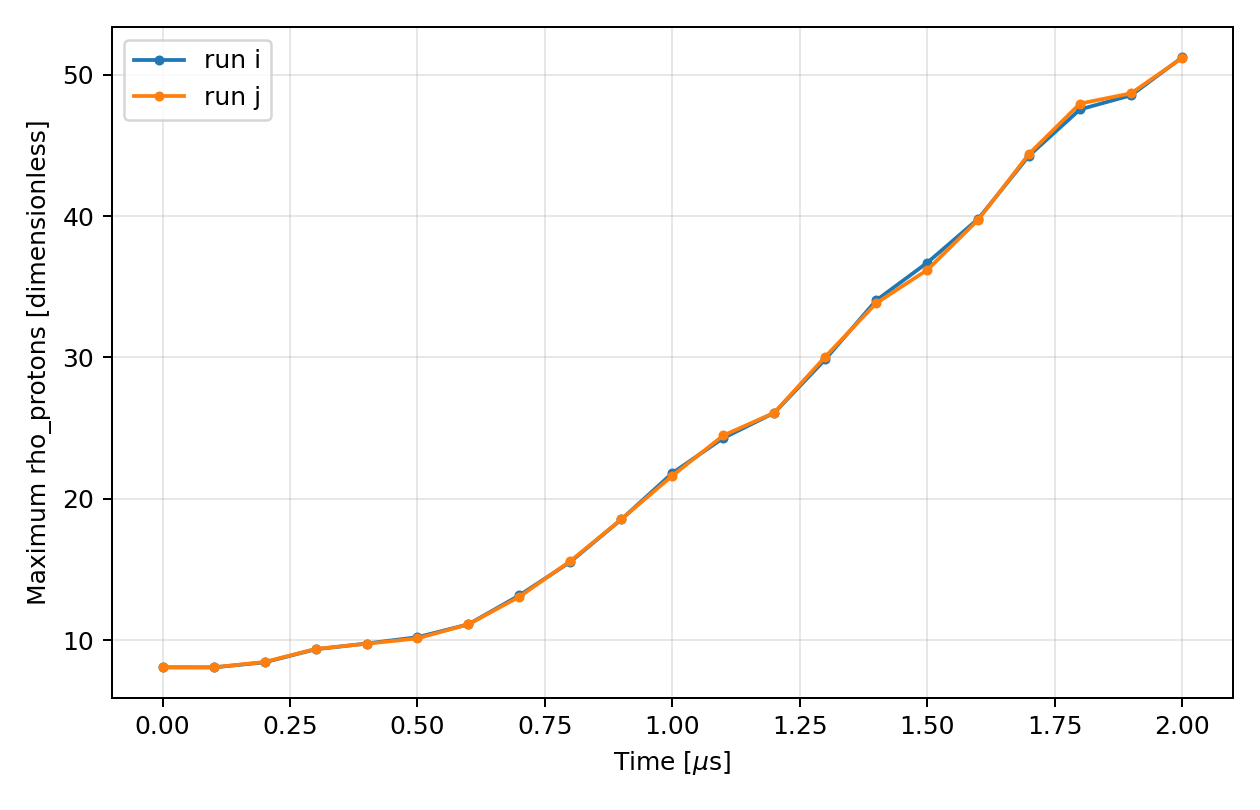
\includegraphics[width=\linewidth]{rho_max_vs_time.png}
        \end{minipage}

        \vspace{0.10cm}
        \begin{minipage}{0.49\linewidth}
            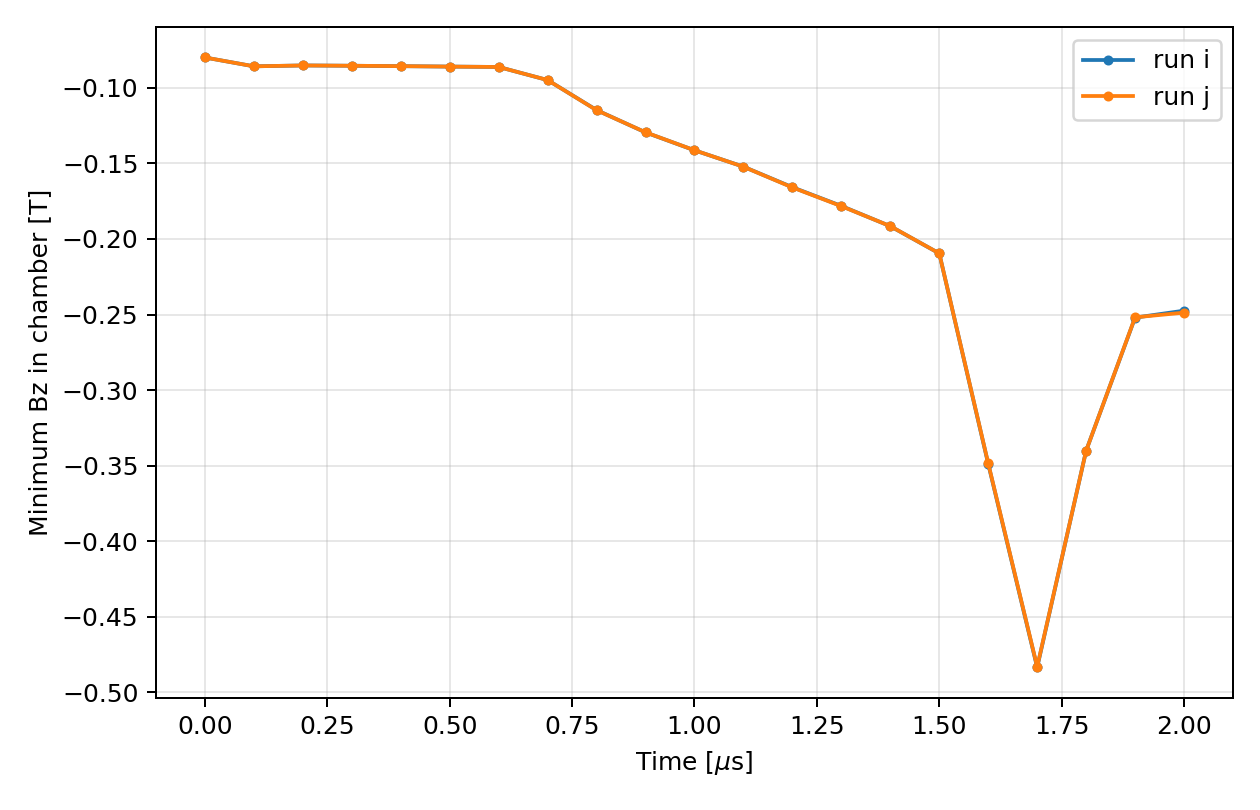
\includegraphics[width=\linewidth]{Bz_min_vs_time.png}
        \end{minipage}
        \hfill
        \begin{minipage}{0.49\linewidth}
            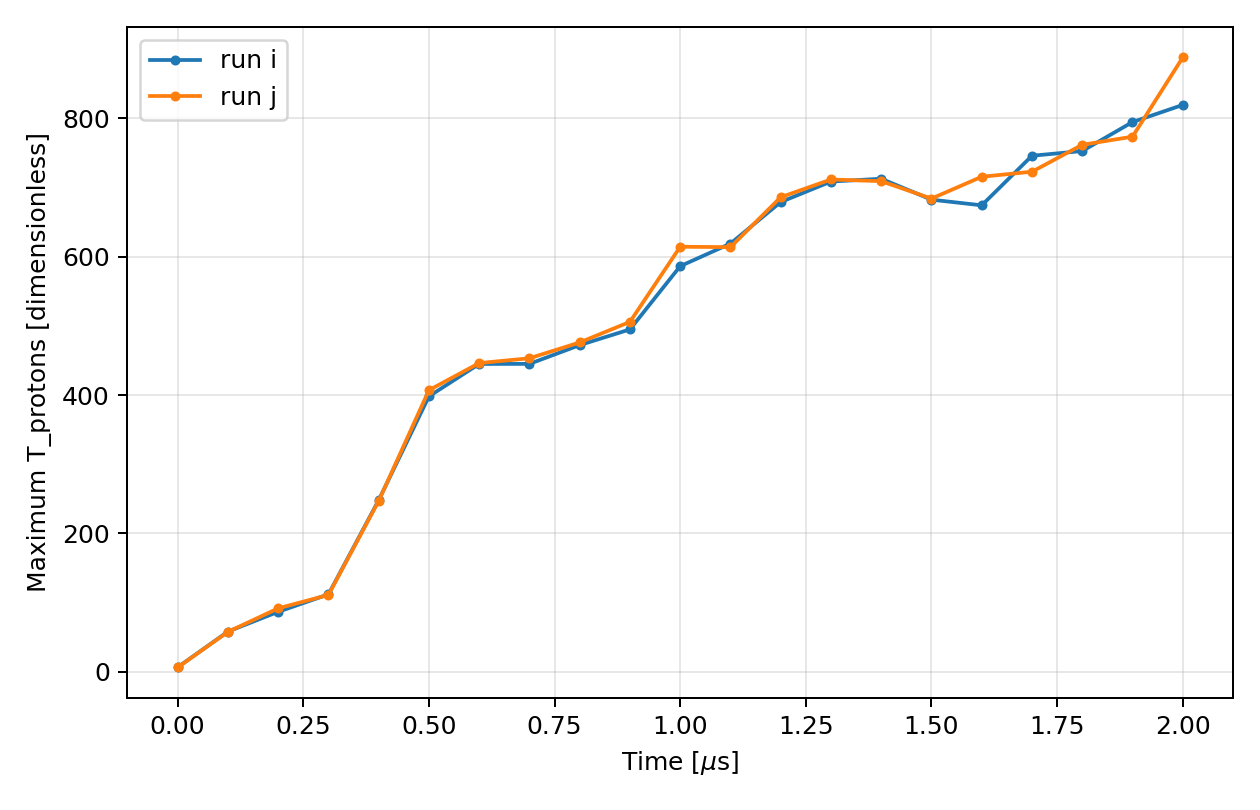
\includegraphics[width=\linewidth]{Ti_max_vs_time.png}
        \end{minipage}
    \end{column}

    \begin{column}{0.40\textwidth}
        \smallcapslabel{Interpretation}
        \vspace{0.08cm}
        \small
        \begin{itemize}\setlength\itemsep{0.14cm}
            \item \texttt{i} and \texttt{j} are not bitwise identical, but their macroscopic evolution is almost the same.
            \item \(B_z\) and density are reliable first regression quantities.
            \item Pointwise \(T_i\) maxima are much noisier and should not be used as strict pass/fail criteria.
            \item Strong magnetic transient appears between \(1.5\) and \(1.8~\mu\mathrm{s}\).
        \end{itemize}

        \begin{beamercolorbox}[wd=\linewidth,rounded=true,sep=0.46em]{neutralbox}
        \scriptsize
        Example run-to-run scale: \\
        \(\max |\Delta B_{z,\mathrm{center}}|\approx3.3\times10^{-4}~\mathrm{T}\).
        \end{beamercolorbox}
    \end{column}
\end{columns}

\end{frame}

% =========================================================
\begin{frame}
\frametitle{Spatial Audit: Development of a Reversed-Field Structure}

\begin{columns}[T,totalwidth=\textwidth]
    \begin{column}{0.49\textwidth}
        \centering
        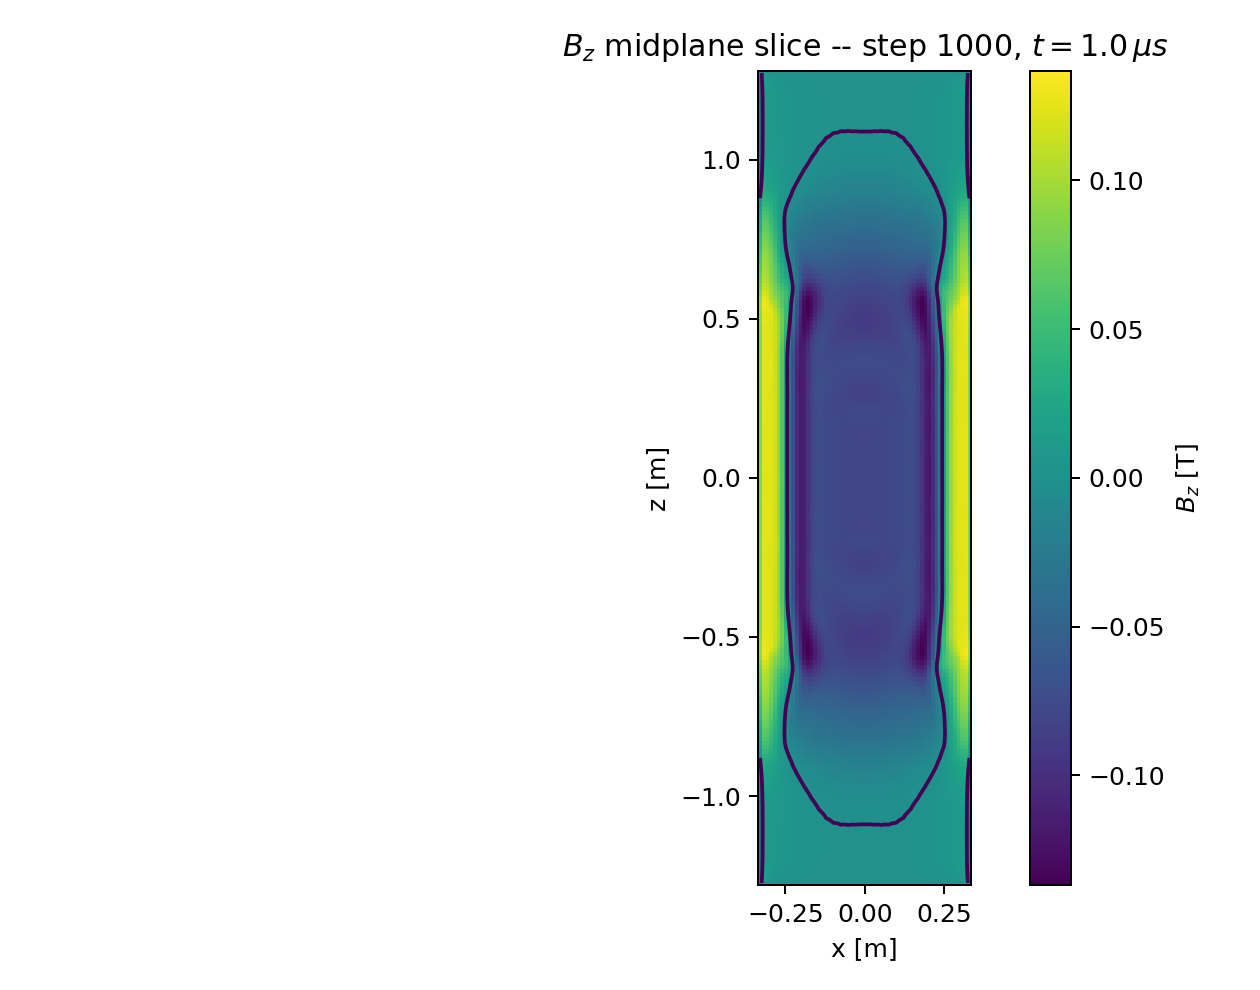
\includegraphics[width=0.86\linewidth]{Bz_xz_step001000.png}

        \vspace{0.04cm}
        {\scriptsize \(t=1.0~\mu\mathrm{s}\): first closed \(B_z=0\) contour in the slice.}
    \end{column}

    \begin{column}{0.49\textwidth}
        \centering
        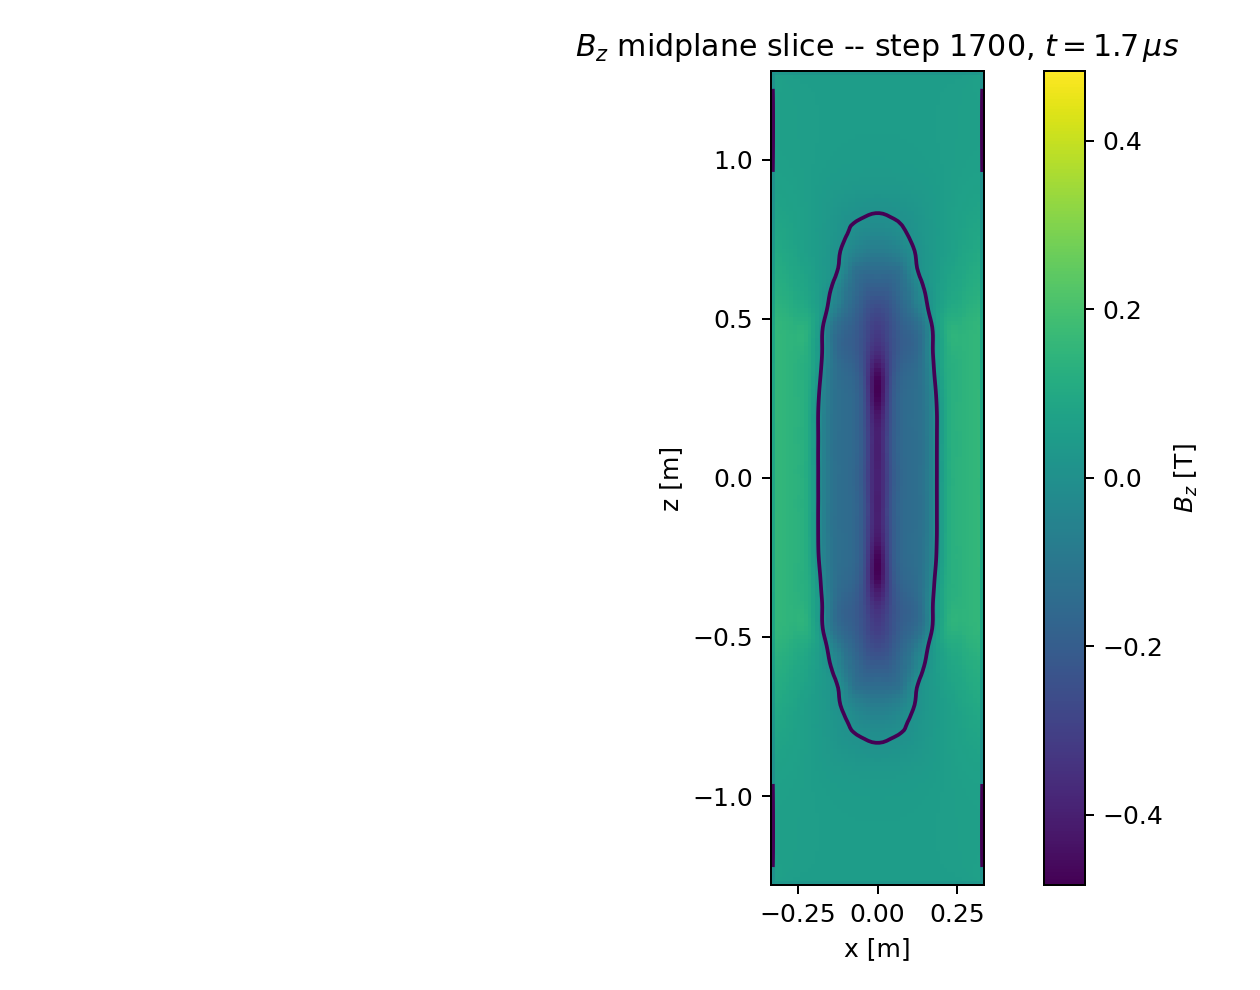
\includegraphics[width=0.86\linewidth]{Bz_xz_step001700.png}

        \vspace{0.04cm}
        {\scriptsize \(t=1.7~\mu\mathrm{s}\): strongest reversed-field compression in the available interval.}
    \end{column}
\end{columns}

\vspace{0.10cm}
\begin{beamercolorbox}[wd=\textwidth,rounded=true,sep=0.44em]{block body}
\scriptsize
The contour shown is \(B_z=0\). It is a useful field-reversal proxy, but it is not yet a rigorous separatrix reconstruction. A proper separatrix estimate should later use the poloidal flux function \(\psi(r,z)\).
\end{beamercolorbox}

\end{frame}

% =========================================================
\begin{frame}
\frametitle{Profiles Confirm the Reversal Is Spatially Extended}

\begin{columns}[T,totalwidth=\textwidth]
    \begin{column}{0.57\textwidth}
        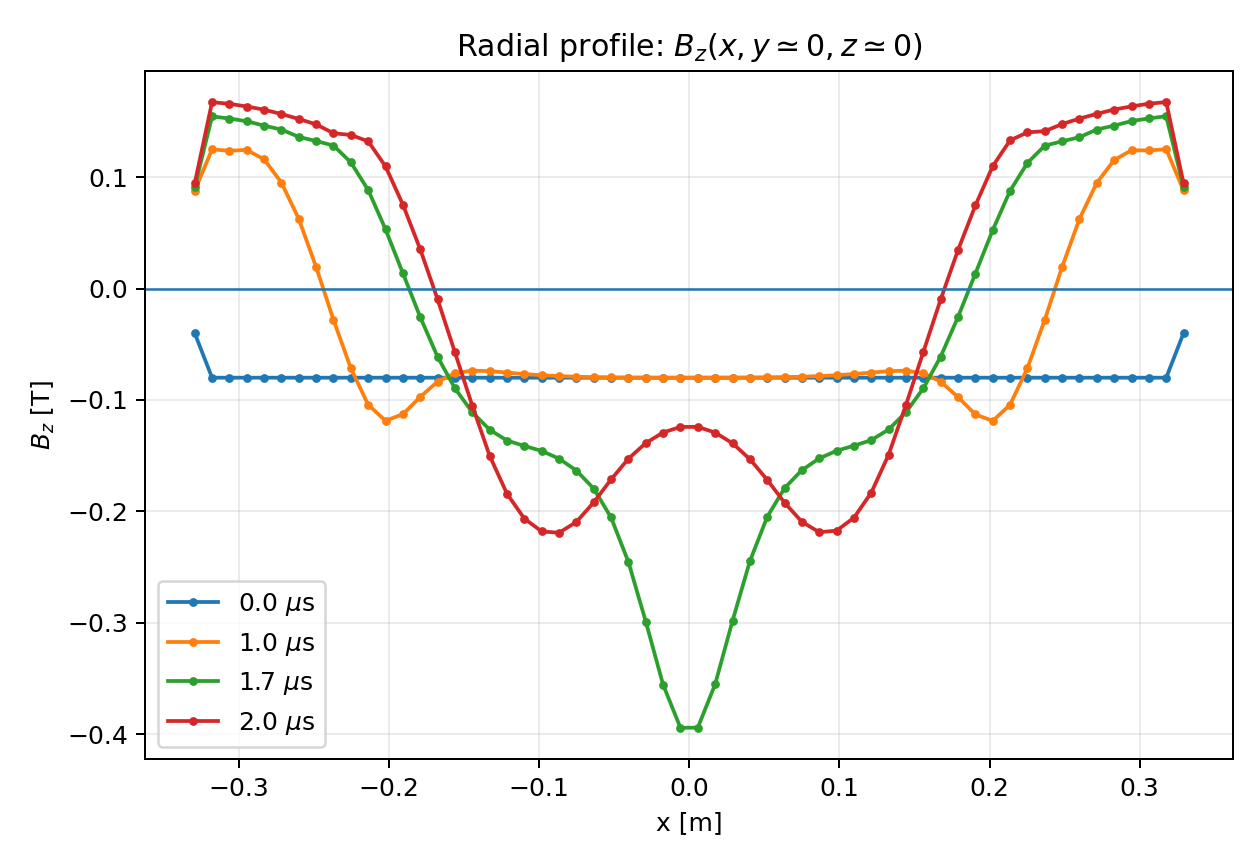
\includegraphics[width=\linewidth]{Bz_radial_profiles.png}

       % \vspace{0.08cm}
        %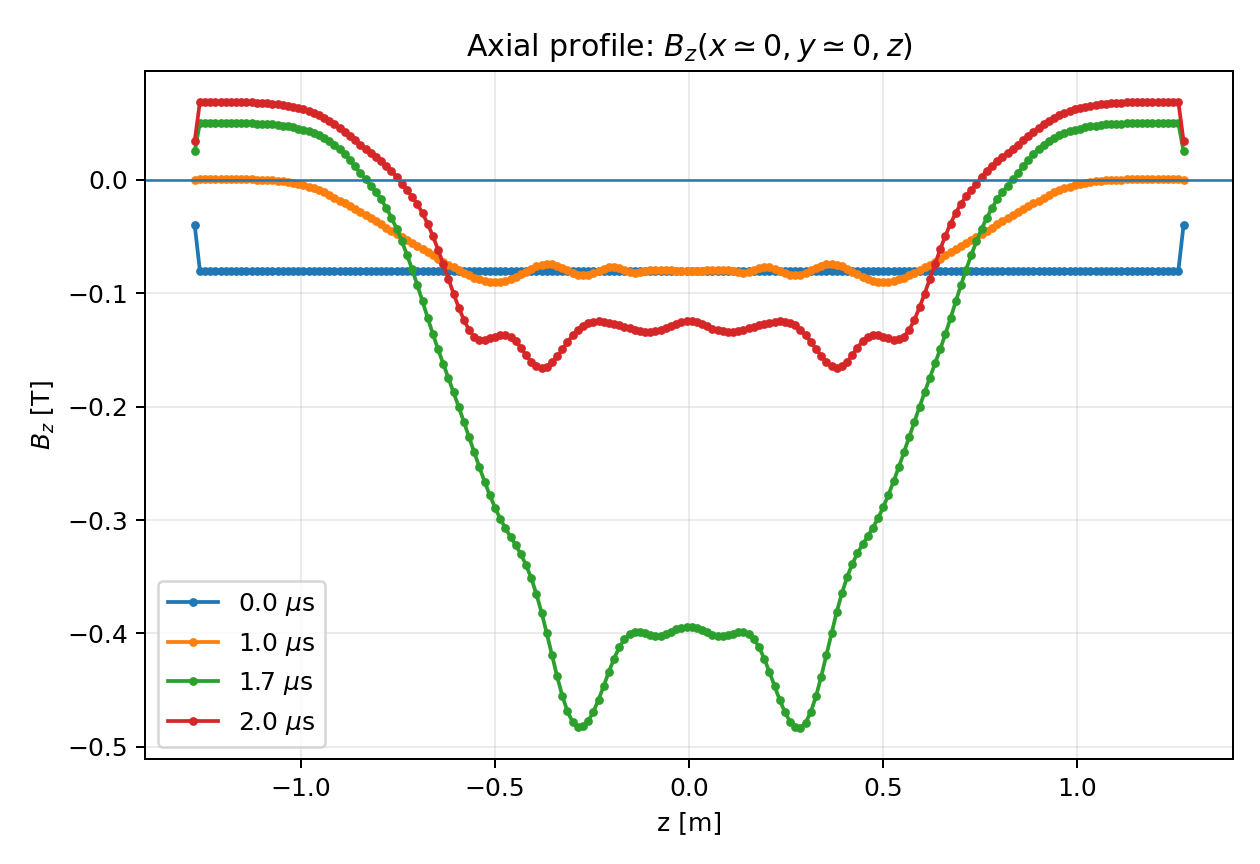
\includegraphics[width=\linewidth]{Bz_axial_profiles.png}
    \end{column}

    \begin{column}{0.41\textwidth}
        \smallcapslabel{What the profiles show}
        \vspace{0.08cm}
        \small
        \begin{itemize}\setlength\itemsep{0.16cm}
            \item Initially, \(B_z\) is negative and nearly uniform inside the plasma region.
            \item By \(1.0~\mu\mathrm{s}\), radial and axial zero crossings appear.
            \item At \(1.7~\mu\mathrm{s}\), the central negative field reaches its strongest value.
            \item At \(2.0~\mu\mathrm{s}\), the reversed structure persists but partially relaxes.
        \end{itemize}

        \begin{beamercolorbox}[wd=\linewidth,rounded=true,sep=0.48em]{donebox}
        \scriptsize
        The field reversal is a coherent spatial feature, not only a single-cell fluctuation or a scalar diagnostic artifact.
        \end{beamercolorbox}
    \end{column}
\end{columns}

\end{frame}

% =========================================================
\begin{frame}
\frametitle{Density Compression Accompanies the Magnetic Evolution}

\begin{columns}[T,totalwidth=\textwidth]
    \begin{column}{0.49\textwidth}
        \centering
        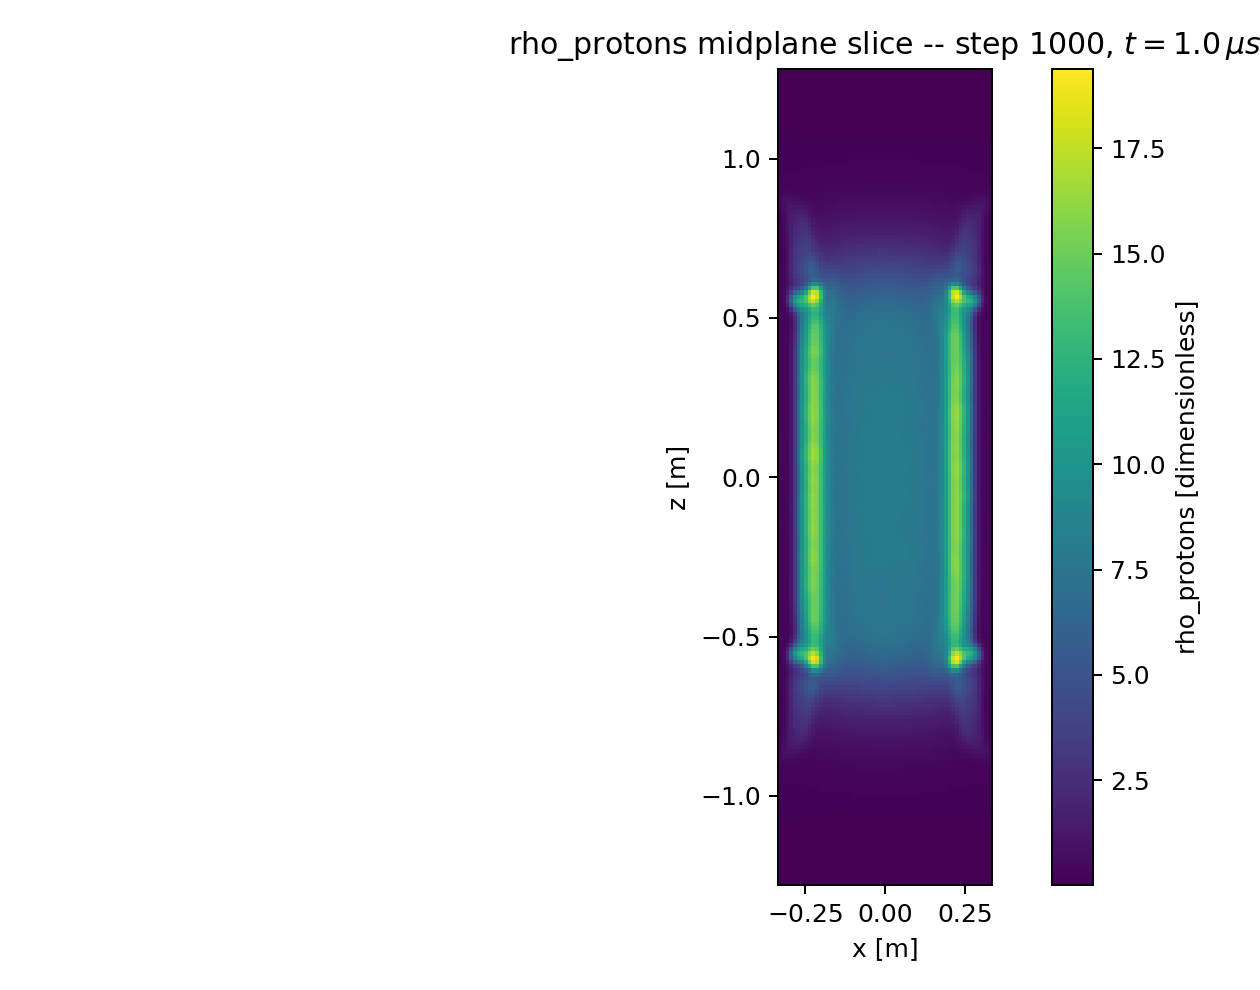
\includegraphics[width=0.88\linewidth]{rho_xz_step001000.png}

        \vspace{0.04cm}
        {\scriptsize \(t=1.0~\mu\mathrm{s}\): density begins to concentrate near the compressed region.}
    \end{column}

    \begin{column}{0.49\textwidth}
        \centering
        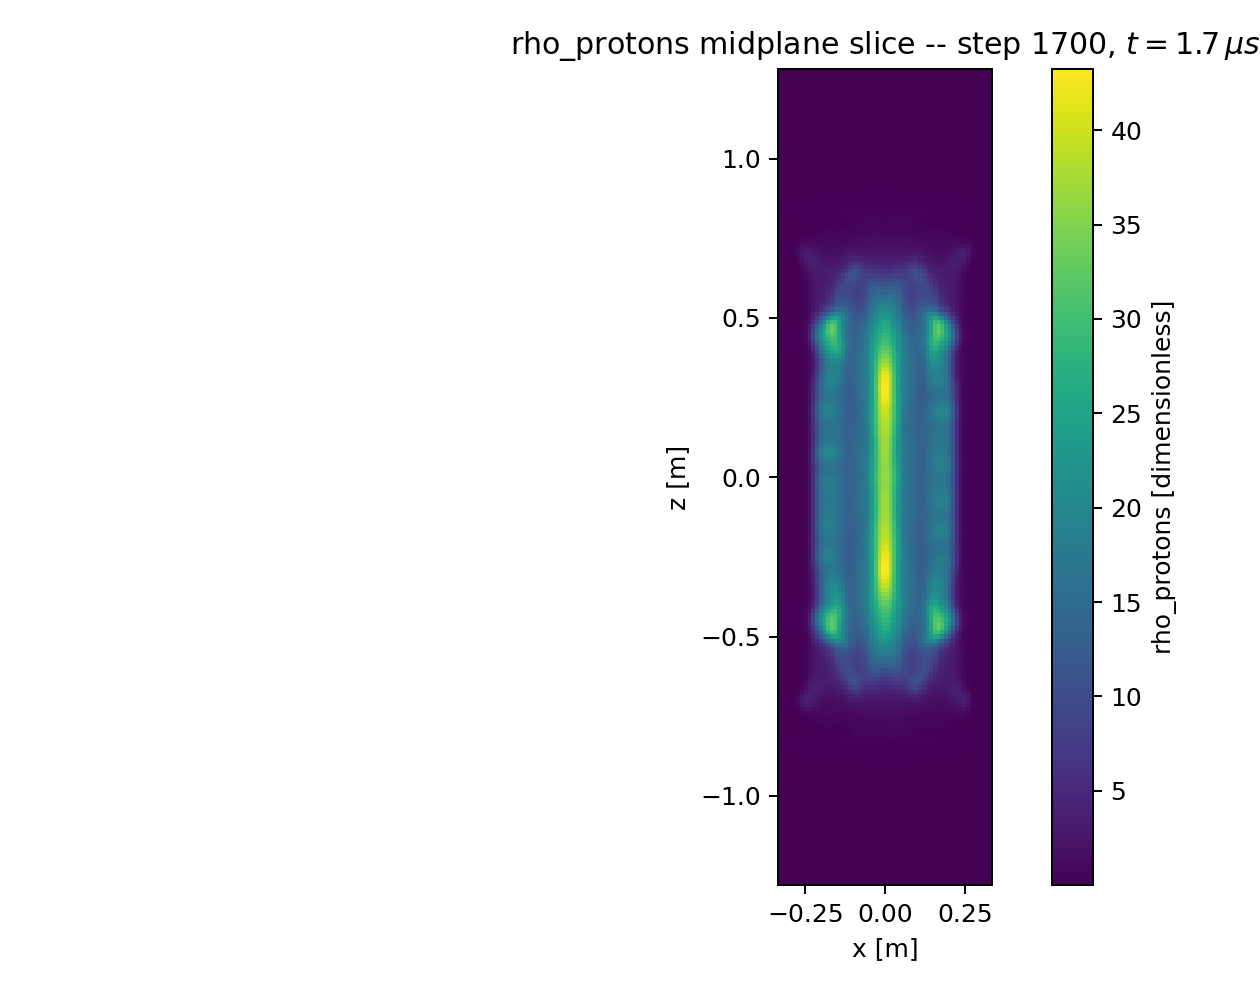
\includegraphics[width=0.88\linewidth]{rho_xz_step001700.png}

        \vspace{0.04cm}
        {\scriptsize \(t=1.7~\mu\mathrm{s}\): strong density enhancement during magnetic compression.}
    \end{column}
\end{columns}

\vspace{0.16cm}
\begin{beamercolorbox}[wd=\textwidth,rounded=true,sep=0.48em]{neutralbox}
\scriptsize
In the central slice, \(\rho_{\max}\) increases from about \(8\) initially to about \(43\) near \(1.7~\mu\mathrm{s}\). The full 3D maximum is larger, indicating that the strongest density point is not necessarily located exactly in the central \(y\simeq0\) plane.
\end{beamercolorbox}

\end{frame}

% =========================================================
\begin{frame}
\frametitle{Current Interpretation of the Inherited Run}

\begin{columns}[T,totalwidth=\textwidth]
    \begin{column}{0.52\textwidth}
        \smallcapslabel{Observed sequence}
        \vspace{0.08cm}
        \begin{beamercolorbox}[wd=\linewidth,rounded=true,sep=0.65em]{block body}
        \small
	\[
	\resizebox{0.96\linewidth}{!}{$
	\boxed{
	\text{bias field}
	\rightarrow
	\text{field reversal}
	\rightarrow
	\text{compression}
	\rightarrow
	\text{partial relaxation}
	}
	$}
	\]
        \vspace{-0.10cm}
        \begin{itemize}\setlength\itemsep{0.10cm}
            \item No reversal at \(t=0\).
            \item Reversal proxy appears by \(1.0~\mu\mathrm{s}\).
            \item Strongest magnetic compression near \(1.7~\mu\mathrm{s}\).
            \item Structure remains visible at \(2.0~\mu\mathrm{s}\).
        \end{itemize}
        \end{beamercolorbox}
    \end{column}

    \begin{column}{0.46\textwidth}
        \smallcapslabel{Important limitation}
        \vspace{0.08cm}
        \begin{beamercolorbox}[wd=\linewidth,rounded=true,sep=0.58em]{nextbox}
        \small
        The existing run is a useful \textbf{regression baseline}, but it is not yet the final scientific formation case.
        \vspace{0.12cm}

        It ends at \(2~\mu\mathrm{s}\), while the applied field reaches its peak only at \(4~\mu\mathrm{s}\).
        \end{beamercolorbox}

        \vspace{0.14cm}
        \begin{beamercolorbox}[wd=\linewidth,rounded=true,sep=0.58em]{neutralbox}
        \scriptsize
        Next scientific target: a longer formation run that reaches and exceeds the full field-rise time, with topology diagnostics such as \(\psi(r,z)\), \(R_s\), \(L_s\), and trapped flux.
        \end{beamercolorbox}
    \end{column}
\end{columns}

\end{frame}

% =========================================================
\begin{frame}
\frametitle{Next Step: Framework v0.1}

\begin{columns}[T,totalwidth=\textwidth]
    \begin{column}{0.49\textwidth}
        \smallcapslabel{Immediate development target}
        \vspace{0.08cm}
        \begin{beamercolorbox}[wd=\linewidth,rounded=true,sep=0.60em]{donebox}
        \small
        Build a minimal reproducible workflow that can generate, submit, and audit a controlled WarpX case without changing the validated physics.
        \end{beamercolorbox}

        \vspace{0.15cm}
        \small
        First components:
        \begin{itemize}\setlength\itemsep{0.11cm}
            \item structured case configuration,
            \item input generation from a template,
            \item Slurm script generation,
            \item run manifest and provenance,
            \item smoke test with very few timesteps.
        \end{itemize}
    \end{column}

    \begin{column}{0.49\textwidth}
        \smallcapslabel{Short-term sequence}
        \vspace{0.08cm}
        \begin{beamercolorbox}[wd=\linewidth,rounded=true,sep=0.65em]{block body}
        \small
        \begin{enumerate}\setlength\itemsep{0.14cm}
            \item Freeze the inherited baseline as read-only reference.
            \item Implement framework v0.1 around the same physics.
            \item Run a cheap smoke test.
            \item Reproduce the inherited 2000-step baseline.
            \item Then extend to a longer scientific formation case.
        \end{enumerate}
        \end{beamercolorbox}
    \end{column}
\end{columns}

\vspace{0.12cm}
\begin{beamercolorbox}[wd=\textwidth,rounded=true,sep=0.44em]{nextbox}
{\scriptsize\textbf{Summary:} the inherited case is now a documented, physically characterized baseline rather than only a collection of old output files.}
\end{beamercolorbox}

\end{frame}

% =========================================================
\begin{frame}[plain]
    \vspace{1.0cm}
    {\color{myblue}\Large\bfseries Summary}\par
    \vspace{0.35cm}

    \begin{beamercolorbox}[wd=0.94\textwidth,rounded=true,sep=0.75em]{block body}
    \small
    \begin{itemize}\setlength\itemsep{0.16cm}
        \item The inherited WarpX/SCNet baseline has been located, preserved, and analyzed.
        \item Runs \texttt{i} and \texttt{j} show reproducible macroscopic FRC-like evolution.
        \item Scalar and spatial diagnostics indicate field reversal, compression, and partial relaxation within the first \(2~\mu\mathrm{s}\).
        \item The next phase is to build a small reproducible framework before launching new physics studies.
    \end{itemize}
    \end{beamercolorbox}

    \vfill
    {\centering\large Thank you\par}
    \vspace{0.6cm}
\end{frame}

\end{document}
